The first, and the simplest method, of scaling pods is \textit{static}
provisioning. Static provisioning requires one wishing to deploy an application on
Kubernetes to determine ahead of time a constant amount of pods for that
application. Any desire to update that static value will require a manual
change. Put simply, with the static method there will be a constant number of
pods, and the application will have a constant amount of resources, throughout
its entire lifetime, regardless of the amount of work the application is asked
to perform.

There are multiple possible heuristics for statically assigning resources to an
applications, as it is possible to over, under, or average provision.

\begin{itemize}
  \item \textbf{Over Provision}: With over provisioning, an application is given
    the greatest amount of resources that it will ever require. With respect to
    horizontal pod auto-scaling, over provisioning means the user of the
    application statically sets the replication controller to ensure that $x$ pods
    always exist, where $x$ is the number of pods needed to
    maintain high quality of service when the application is
    asked to perform the most work.\footnote{In this discussion, references to
      \textit{most}, \textit{least}, and \textit{average} work assume that there
      exist bounds on the work the external environment can ask the application to
      do.} While over provisioning ensures a high quality of service, it has extremely
      poor efficient resource utilization, as can be seen in Figure
      \ref{fig:static-over-provision}.

    \begin{figure}[!h]
      \centerline{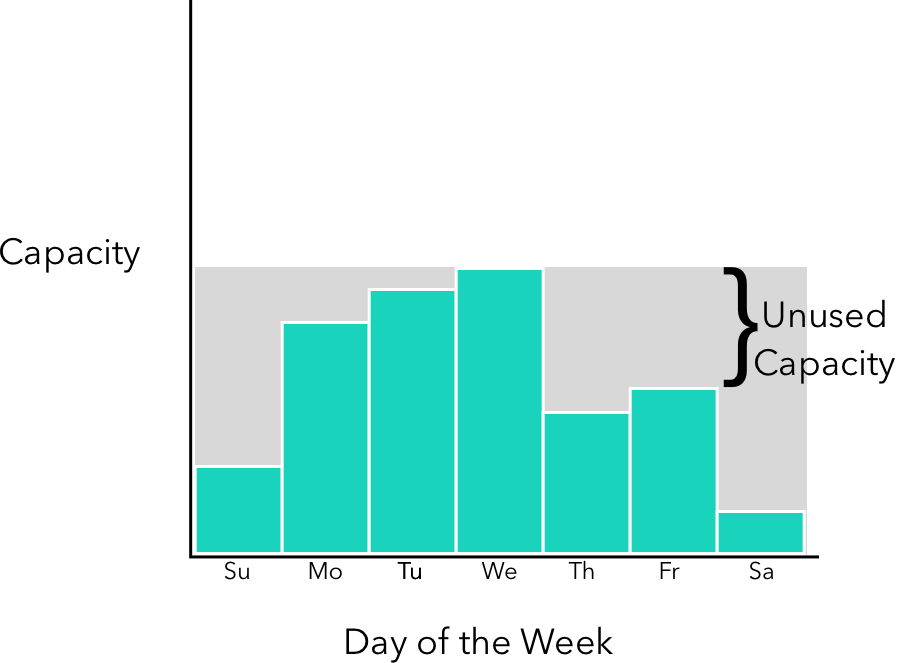
\includegraphics[scale=.25]{static-over-provision.jpg}}
      \caption{A Over Provisioned Application}
      \label{fig:static-over-provision}
    \end{figure}

  \item \textbf{Under Provision}: With under provisioning, an application is
    given the least amount of resources that it will ever require. Again, in the
    context of horizontal pod auto-scaling, under provisioning leads to user to
    statically set the replication controller to ensure the existence of
    $y$ pods, where $y$ is the number of pods needed to maintain quality of
    serice when the application is asked to perform the least work. Under
    provisioning ensures efficient resource utilization, as the application will
    never reserve any resources and then leave them idle. However, in all
    situations except for when the application performs the minimum possible
    amount of work, quality of service will suffer because the application does
    not have enough resources.

  \item \textbf{Average Provision}: With average provisioning, an application is
    given the average amount of resources that it needs. With respect to
    horizontal pod auto-scaling, average provisioning guides the user to
    statically set the replication controller to maintain $z$ pods, where
    $z$ is the number of pods needed to maintain quality of service when the
    application is asked to perform the average amount of work. Average
    provisioning can be seen as somewhat of a middle ground between under and
    over provisioning, offering decent quality of service and efficient resource
    utilization, as can be seen in Figure \ref{fig:static-average-provision}.

    \begin{figure}[!h]
      \centerline{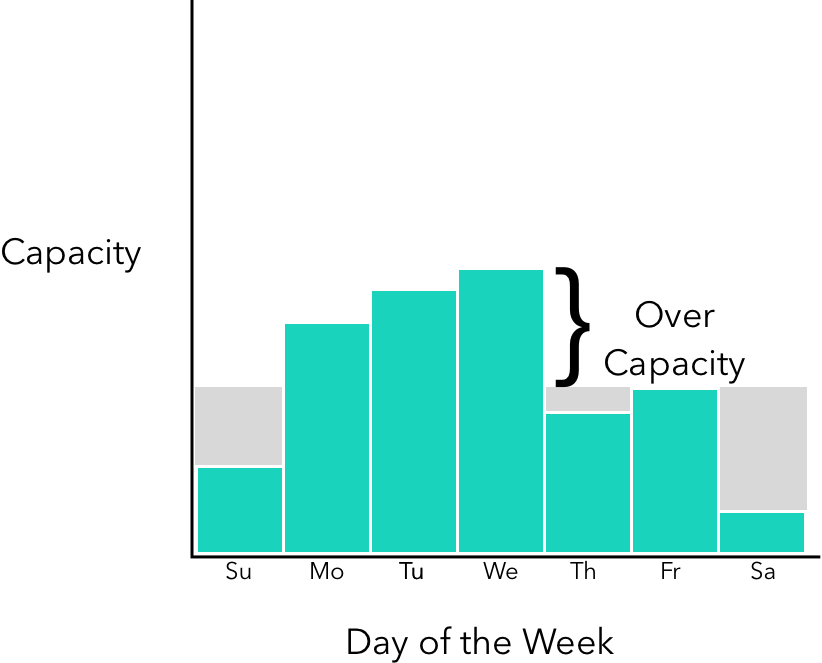
\includegraphics[scale=.25]{static-average-provision.jpg}}
      \caption{A Average Provisioned Application}
      \label{fig:static-average-provision}
    \end{figure}
\end{itemize}

Our discussion of static provisioning in Kubernetes makes the assumption that
creating a static number of pods equates to reserving a static amount of
resources. In the default case, the previous statement is not necessarily true,
yet it is possible to craft specialized pods which validate this equality. To
start, remember that pods contain containers. When Kubernetes receives a pod, it
seeks to schedule all of its containers on a physical node within the cluster.
By default, containers within the pod run with no bounds on their CPU and memory
beyond the constrictions the physical node on which they are scheduled. As such,
declaring $x$ number of pods does not give any guarantees of resource usage, as
the amount of resources available to the containers within the pod vary
drastically based on their specific node \cite{k8s-limit-range}. This variability challenges the
stability of static provisioning, and weakens its ability to serve as a control
group with which we can compare predictive horizontal auto-scaling.

Fortunately, there is a way to modify configure Kubernetes such that a static number of
pods equates to a static number of resources.\footnote{Right now in Kubernetes,
resources relates to either CPU or memory. CPU is requested in cores. Memory is
requested in bytes of RAM.} This configuration involves
setting resource requests and limits for each container within the pod. A
resource request for a container indicates the minimum amount of resources that
should always be available. A pod will not be scheduled on a node within the
cluster, unless that node can guarantee the requested amount of resources to all
containers within the pod. A resource limit for a container indicates the
maximum amount of resources that a container can claim. Depending on the
resource, a container exceeding the maximum amount of resources will either be
throttled (CPU) or killed (memory).\footnote{It is also possible to configure
Kubernetes such that a container using too much CPU is killed.} A pod's resource
request\/limit is the summation of the resource request\/limit for all of its
containers. Setting a container's, or pod's, resource request equal to its
resource limit essentially guarantees that the existence of a pod represents the
claiming and utilization of a static amount of resources
\cite{k8s-compute-resources}. Ensuring static provisioning
is reserving a consistent amount of resources
allows us to still examine idle CPU percentage, our way of investigating
efficient resource utializaiton. We additionally incorporate similar CPU limits
and requests when testing reactive and predictive auto-scaling, again because it
makes it easier to reason about idle CPU.

In the interest of reducing the amount of length evaluation jobs that we run,
perform one test in which we compare average static provisioning, reactive
auto-scaling, and predictive auto-scaling for a single test pattern and pod
initialization time. Ultimately, we do not devote significant time to
considering any type of static provisioning, as we are confident that it will at
best be equal to reactive auto-scaling. Thus if our implementation of predictive
auto-scaling outperforms reactive auto-scaling, we are confident that it will
also outperform any type of static provisioning.
